

\chapter{基于区域合并的图像显著性分析算法}
\label{ch2:SGRM}
本章提出了一种显著性引导的图像区域合并算法,用于图像显著性区域检测。算法的目标是直接通过区域合并的方式逐渐将图像从初始状态下的多个区域合并为显著性对象和背景2个区域。为实现这一目标,在不同的阶段采用不同的合并策略。首先利用超像素分割方法将图像分为若干初始区域。在第一阶段,仅合并相似且相邻的区域,使得属于同一对象的像素合并到同一区域;随后进行第二阶段合并,处理上述过程中产生的空洞以及因遮挡造成的属于同一对象的区域不相邻的情况;在第三阶段合并时,以区域显著分析结果为引导,不断将显著性最差的区域合并到背景区域,而不是尝试将显著性区域合并到一起;最后,利用合并过程中得到的多个候选显著性区域加权得到最终的显著性区域结果。为了验证算法的有效性,在2个国际上公开的测试集ASD~\cite{Achanta08}和ECSSD~\cite{ECSSD}上测试了本章所提算法,并与其它同类算法进行了对比。实验结果证明了本章所提算法的有效性,特别是在难度更大的ECSSD数据集~\cite{ECSSD}中,本章算法的准确度要优于其它同类算法。
\section{研究背景}
\label{sec:background}
图像显著性区域检测是近年来计算机视觉和图像处理领域的研究热点之一~\cite{saliencySurvey}。该技术的目标是快速定位图像中显著性对象,可以广泛应用于目标识别,基于内容的图像编辑以及图像检索等应用中。早期的显著性检测算法~\cite{itti}依据视觉感知理论,采用自底向上方法预测人眼观察图像时的焦点(fixation),最终得到一系列离散的圆点形状的显著性区域预测结果。然而,这类方法效率和准确度均较低,且无法得到显著性对象的准确边界,实际应用范围受限。随后,为了实现提前显著性对象的准确边界,研究人员提出了一系列数据驱动,自底向上的显著性区域检测算法~\cite{Achanta08,ChengPAMI,ufo,Yan2014Hierarchical},大大提高了显著性对象检测精度以及计算速度。目前这类算法均可以较为准确的提取自然图像中包含的显著性对象,实现显著性对象与背景的分离。\par
据文献~\inlinecite{Borji2015Salient}报道,在这些算法中,基于图像区域的算法性能更出色。基于区域的显著性检测算法首先用超像素~\cite{SLIC}、基于图的图像分割算法~\cite{graphseg}等图像分割方法将图像分为若干个小区域,随后以区域为单位进行显著性计算。由于在区域分割时考虑了像素在色彩以及空间域的连续性,分割后的区域内像素具有很好的齐次性,且大部分区域之间的边界与图像边缘吻合。 相比于基于像素的算法, 区域分割处理在保持显著性对象边界的同时,可以利用区域颜色直方图更准确的对区域内的颜色对比度进行量化。另外,以区域为单位计算大大降低了运算量。\par
当前大部分已有的图像显著性检测算法的出发点均是根据显著性区域的特点,例如对比度高~\cite{ChengPAMI}、处在相机焦点上~\cite{ufo}等,定义区域显著性模型以计算每个像素的显著性水平。然而,自然图像中可能包含各种类型的显著性对象,单纯用这些显著性对象的线索仍然无法处理所有情况。如图~\ref{fig:saliencyCom}所示,(a)为输入图像,(b)、(c)、(d)分别为CHS算法~\cite{Yan2014Hierarchical}、RC算法~\cite{ChengPAMI},和本章算法的结果,(e)为正确结果。图~\ref{fig:saliencyCom}表明,当输入图像中对象和背景的色彩分布较为接近(图~\ref{fig:saliencyCom}中第一行和第二行),或者背景复杂度较高(第三行)时RC和CHS算法均无法有效检测出显著性对象。
\begin{figure}[htb]
  \centering%
      {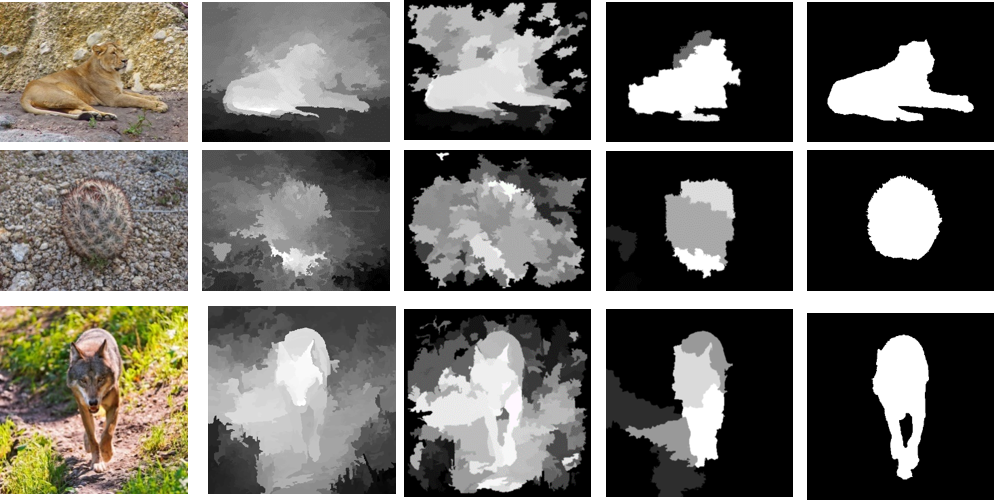
\includegraphics[width=0.9\textwidth]{ch2/ch02fig1.png}}\\
(a)\quad\quad\quad\quad\quad
(b)\quad\quad\quad\quad\quad\quad
(c)\quad\quad\quad\quad\quad\quad
(d)\quad\quad\quad\quad\quad
(e)
  \caption{显著性检测结果对比}
  \label{fig:saliencyCom}
\end{figure}

\par
为了解决这一问题,本章将显著性区域检测问题视为图像分割问题,以显著性引导的区域合并的方式将图像分为显著性区域(前景)和背景两个区域。在合并过程中采用了与主流基于区域的图像显著性检测算法~\cite{Achanta08,ChengPAMI,ufo,Yan2014Hierarchical}相反的策略,即不再尝试定位显著性区域,而是利用背景线索来估计背景区域,并不断将显著性差的非前景区域合并到背景区域。根据观察,大部分自然图像中的背景部分的像素具有连续性强的特点~\cite{huamiao},例如室外拍摄图像中的天空,地面等背景区域。此外,图像的边缘部分应该大部分都是背景~\cite{backgroundPrior}。如果不断将图像中相似的小区域进行合并,背景部分像素应该更容易合并到一起,并且将包含更多的图像边缘。观察图~\ref{fig:saliencyCom}中输入图像的背景部分,如第一行图像中的地面以及狮子身后的山、第二行图像中的石块地面、以及第三行图像中的草地,虽然这些背景部分色彩分布与前景接近或者具有较高的复杂度,其仍然具有这种较强的连续性。在区域合并时本文没有尝试将显著性区域合并到一起,而是利用背景区域线索,首先将图像进行超像素分割,随后在区域显著分析的引导下不断将显著性最差的区域合并到背景区域。最后,利用合并过程中得到的多个候选显著性区域加权得到最终的显著性区域结果。将本章算法在两个公开的数据库ASD~\cite{Achanta08}和ECSSD~\cite{ECSSD}中的共计2000张图像中进行了测试并与其它算法进行了对比,实验结果验证了本章所提算法的有效性。在较为困难的ECSSD测试集中,本章算法得到的F-Mearsure以及平均绝对误差(MAE)均优于其它参与比较的相关算法。

\section{相关工作}
\label{sec:relatedWorks}
\subsection{图像显著性区域检测}
\label{sec:SaliencyDetection}
对比度(contrast)强是显著性对象区别于背景的重要性质,Cheng等人~\cite{ChengPAMI}提出利用全局对比度的方法计算图像中每个颜色的显著性水平。由于色彩空间巨大,为了提高效率,Cheng等人提出量化的方式提取图像中的主要颜色并依据此建立直方图,计算每个颜色的显著性值。为了进一步提高算法的准确的,Cheng等人~\cite{ChengPAMI}提出了一种基于区域对比度的方法,先用基于图的图像分割方法将图像分为若干齐次区域,考虑区域的空间相关性,利用区域对比度来检测显著性区域,得到了比全局对比度更好的效果。Perazzi等人~\cite{saliencyFilter}提出基于高维高斯滤波的显著性滤波算法(saliency filters)。该算法首先对待处理图像进行抽象化,去掉冗余细节信息。随后在CIELab色彩空间中通过局部及全局对比度来计算色彩独特性,利用高维高斯滤波的方式结合色彩的空间分布情况计算最终的显著性检测结果。Jiang等人~\cite{ufo}指出,作为主要目标显著性对象应该在成像时处于相机焦点之上,利用图像中边缘的模糊程度可以对图像区域是否在成像时处于相机的焦点上进行量化,最后综合考虑图像区域对比度、是否在相机焦点上以及区域中包含对象的可能性(objectness)三方面线索计算最终的结果。Li等人~\cite{DSR}提出一种基于重建误差的显著性检测算法, DSR。 该算法首先利用超像素提取图像的边界, 计算每个区域的稠密及稀疏重建误差; 随后利用$K$-means算法对重建误差信息进行聚类, 最后通过多尺度重建误差集成和偏向对象的高斯模型优化得到像素级的显著性结果。 Jiang等人\cite{MC}提出一种基于图像图模型上的吸收马尔可夫链的算法, 该方法结合了显著性对象的独特性和背景区域的空间分布特点等线索, 利用马尔可夫链模型中各节点至边界吸收节点的吸收时间来评估像素的显著性。 为了处理自然图像中的复杂结构,Yan等人~\cite{ECSSD}提出了一种多尺度参差花的显著性区域检测算法,称为CHS。该方法将图像在不同尺度上进行分割,得到多个层次的区域显著性线索,并将这些多层次的线索进行加权得到最终结果。本章所提出的方法与CHS算法有类似之处,均采用了图像区域合并的方法得到多个图像分割结果。但不同之处在于本章提出的区域合并方法在合并过程中的不同阶段使用不同的合并策略,而CHS算法使用同样的分层策略得到固定数量的层次。并且,本章使用背景线索进行区域显著性分析,与上述基于显著性对象线索的算法均不同。\par
Wei等人~\cite{geodesicDistance}提出了一种基于背景线索的显著性检测算法,该方法利用背景部分像素容易连接到图像边界的特点,利用图像区域距离图像边界的测地线距离(geodesic distance)来评估其显著性。文献~\inlinecite{backgroundPrior}中利用了图像边界大部分是背景这一假设,先对图像边界区域进行对比度分析,从中获得背景区域主要颜色的线索;随后利用这一线索利用基于~\inlinecite{ChengPAMI}的算法进行对比度分析获得显著性前景结果。本章算法基于类似的背景线索,但是本章所提算法通过显著性引导的区域合并的方式进行显著性检测,这与文献~\inlinecite{geodesicDistance,backgroundPrior}有较大差别。\par
与基于区域的算法不同, Wang等人~\cite{PISA}提出一种基于像素的显著性检测算法, PISA。 该算法主要利用图像全局范围内的颜色和结构对比度及其在图像空间域中的分布情况等线索,以滤波的方式将多种线索合成得到图像中每个像素的显著性值。虽然PISA算法的准确度与本章算法较为接近,但是由于PISA是基于像素的算法,本章算法与之相比在速度上有明显优势。

\subsection{图像区域合并}
\label{sec:regionMerging}
图像区域合并是指根据图像区域之间的相似性,逐渐将相似的区域合并在一起的过程,常用于图像分割等应用中。Richard~\cite{Richard2004Statistical}提出了一种基于统计的区域合并的图像分割算法,利用图像统计特性确定需要合并的区域以及合并的顺序。在算法的初始阶段,每个像素表示一个区域,以相邻区域间颜色的差值的升序进行排序。在合并过程中,按此顺序将区域间颜色差距在门限之内的区域进行合并,直到剩余的区域数量达到合并要求。文献~\inlinecite{Xiao2015Complexity}提出了一种复杂度自适应的图像区域距离以衡量图像区域的相似性,并以之为基础评估区域间的相似性。在合并时,优先合并相似区域。在区域合并完成后,根据区域中包含边缘信息的情况来评估区域中包含对象的可能性(objectness)。文献~\inlinecite{SelectiveSearch}中提出了一种基于贪心算法的图像区域合并方法,该方法不断合并所有邻居区域中最接近的两个区域,直到将整幅图像合并为一个区域。上述区域合并方法作为预处理方法用于对象识别和显著性区域检测算法中取得了不错的效果。但上述方法均在区域合并过程中均始终采用同一策略,没有考虑到区域合并过程中不同阶段的不同特点,容易将属于对象的像素合并到背景区域。\par
如图~\ref{fig:rm}所示,图~\ref{fig:sub:img}为输入图像,其中水面上划船的人为显著性前景对象。分别利用文献~\inlinecite{Richard2004Statistical}、~\inlinecite{Xiao2015Complexity}所提出的图像区域合并算法对输入图像进行分割,得到结果如图~\ref{fig:sub:srm}和图~\ref{fig:sub:cadm}所示。输入图像被分为9个区域,分别用不同的随机颜色表示。从图中可以看出,当分割进行到此阶段时,文献~\inlinecite{Richard2004Statistical}、~\inlinecite{Xiao2015Complexity}算法会将前景对象合并到背景区域中。其中图~\ref{fig:sub:cadm}中结果更为明显,划船人被分割到多个区域中。出现这种情况的主要原因是在合并过程中随着区域逐渐扩大区域间的相似度越来越高,如果在合并时只考虑区域间在色彩及空间上的相似度则很容易将属于前景区域与属于背景的区域合并到一起。另外,前景对象一般具有连续和紧凑的特点,即属于前景的对象的空间分布较为集中。如果在合并时仅允许相邻的区域进行合并~\cite{SelectiveSearch}可以在一定程度上防止前景区域合并到背景区域。但是考虑到前景对象对背景的遮挡,又会使得背景区域无法合并到一起。例如,图 ~\ref{fig:sub:img}中输入图像中背景部分的树林,由于前景对象的遮挡,这部分区域不再联通。一个理想的区域合并算法应该能处理好上述问题,使得属于前景区域和背景区域的像素能分别合并到一起。与这些方法不同,本章所提算法的目标是将图像分为显著性对象和背景2个区域,且在不同的阶段采用不同的合并策略,可以避免在合并过程中误将显著性对象合并到背景区域。
\begin{figure}[htb]
  \centering%
  \subcaptionbox{输入图像\label{fig:sub:img}} %标题的长度,超过则会换行,如下一个小图。
    {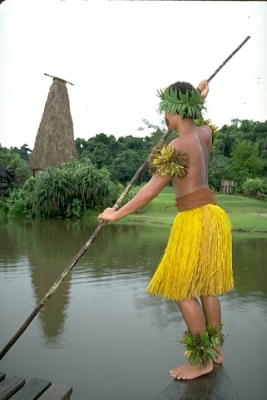
\includegraphics[width=0.25\textwidth]{ch2/0001.jpg}}%
 \hspace{1em}%
  \subcaptionbox{~\inlinecite{Richard2004Statistical}分割结果			   \label{fig:sub:srm}}
      {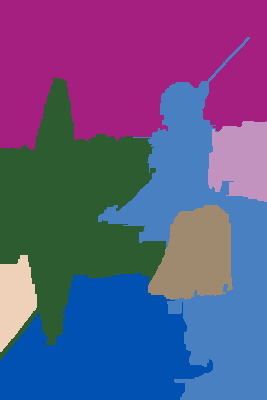
\includegraphics[width=0.25\textwidth]{ch2/srm_7.png}}
 \hspace{1em}
  \subcaptionbox{~\inlinecite{Xiao2015Complexity}分割结果\label{fig:sub:cadm}}
      {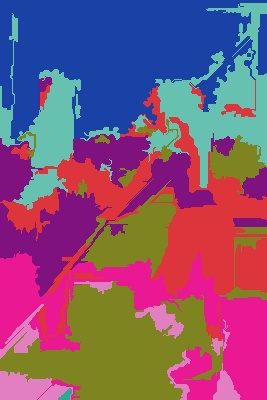
\includegraphics[width=0.25\textwidth]{ch2/cadm.jpg}}
  \caption{基于区域合并的图像分割结果比较}
  \label{fig:rm}
\end{figure}


\section{算法描述}
\label{sec:algorithm}
本章算法主要分为三个阶段,主要流程图如图~\ref{fig:algflow}所示。首先,依据像素的空间相关性和色彩一致性利用文献~\inlinecite{superpixel}的算法对图像进行超像素分割, 将图像分为多个初始区域。 随后,开始第一阶段合并,在此阶段不断将相似的相邻区域进行合并,直到区域数量达到阈值$N$。由于前景的遮挡,可能会使某些背景区域被分割成多个小区域,同时在前一过程中会有一些小区域由于与周围区域差别较大无法参与合并而形成空洞。在第二阶段处理这些遮挡和空洞问题,允许相似但不相邻的区域进行合并,同时将空洞区域与其最相似的邻居区域进行合并。在第三阶段,采用显著性引导的合并策略,分析各区域的显著性,将显著性最差的区域标记为背景区域$R_{B}$,剩下的其它区域一起可以看作是可能的显著性区域。不断以显著性从低到高的顺序依次将所有区域合并到$R_{B}$。最后将在合并过程中可以得到的候选显著性区域(proposals)加权平均得到最终显著性区域结果。\par
\begin{figure}[htb]
  \centering%
      {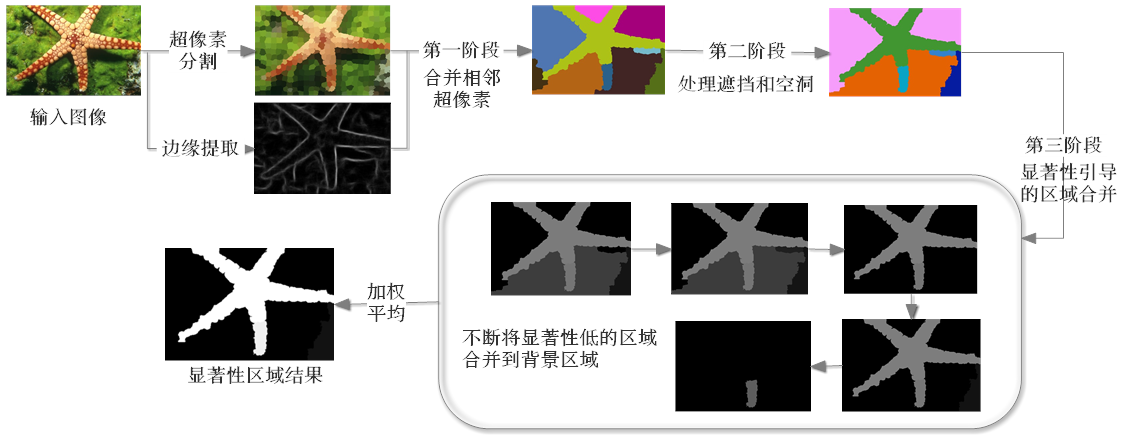
\includegraphics[width=0.9\textwidth]{ch2/SGRMflowChart.png}}

  \caption{算法流程图}
  \label{fig:algflow}
\end{figure}

\par
下面分别详细介绍各阶段的合并规则。

\subsection{第一阶段合并}
\label{subsec:mergeP1}
第一阶段合并只允许相似且相邻的区域进行合并。将区域$i$与区域$j$的合并优先级定义为$PR(i,j)$。计算区域合并的优先级时考虑以下四项因素。
\begin{itemize}
\item 颜色相似性\par
    直观上看,色彩分布一致的区域属于同一对象的概率很大。利用区域颜色直方图的巴氏距离(bhattacharyya distance)来量化区域之间的色彩相似性,越相似的区域合并优先级越高。

    \begin{equation}
    \label{equ:chap2:Pc}
    P_{c}(i,j)=1-HistogramDist(i,j)
    \end{equation}
    其中$HistogramDist$为计算直方图巴氏距离的函数。为了提高效率,利用文献~\inlinecite{ChengPAMI}中提的直方图量化方法对图像色彩空间进行简化处理。在保证覆盖图像中$95\%$以上像素颜色的情况下,去掉图像中出现频次较低的颜色,从而减少直方图的分块(bin)数量以减少计算量。大部分图像在经过处理后的颜色直方图大约包含1000个左右分块。
\item 边缘保持\par
    图像结构化边缘是反映对象边界的重要信息。为了使区域合并过程不破坏对象的边界,在合并优先级中加入边缘保持项,降低区域间的边界包含图像边缘的区域对的优先级。具体其定义为:
    $$P_{e}(i,j)=1-\frac{E(i,j)}{min(borderLen(i),borderLen(j))}$$
    其中$E(i,j)=\sum_{b\in border(i,j)}Edgeness(b)$,即区域$i$和$j$之间的边界的边缘响应之和, $borderLen(i)$表示区域$i$ 边界的长度(像素数)。本章算法利用文献~\inlinecite{DollarEdge}所提出的算法计算图像的结构化边缘响应,并将其归一化到$[0,1]$之间。
\item 区域空间相关性\par
    区域的空间相关性指区域在空间上的关联性,对于相邻的区域其相关性定义为$$P_{s}(i,j)=borderLen(i,j)/min⁡(border(i),border(j))$$,其中 $borderLen(i,j)$表示区域$i$和$j$之间边界的长度。区域空间相关性的几何意义为若两区域之间的边界占比越大,说明两区域在空间关系上关联更紧密,因此合并优先级更高。极限情况下,当区域$i$ 完全包含$j$时$P_{s} (i,j)=1$。
\item 区域面积\par
    为了使区域合并在图像全局范围内进行,对面积较小的区域赋予较大优先级。在合并过程中,图像中那些与周围邻域差距较大的区域因为无法进行合并而产生空洞。在合并时考虑区域面积,可以在一定程度上减少空洞的出现。区域面积项的具体定义为:
    $$P_{si}=1-(size(i)+size(j))/TotalSize$$
其中$TotalSize$是图像的总像素数,$size(i),size(j)$表示区域$i,j$的像素数。
\end{itemize}
最终, $PR(i,j)$由上述四项加权平均得到:
\begin{equation}
   \label{equ:chap2:PR}
   PR(i,j)=w_{c}\times P_{c}+w_{e} \times P_{e} + w_{s} \times P_{s} + w_{si} \times P_{si}
\end{equation}
其中加权系数$w_c=0.5, w_e=0.1, w_s=0.2, w_{si}=0.2$为固定值。\par

第一阶段合并过程的具体算法如算法~\ref{alg:algMergeP1}所示。



\renewcommand{\algorithmcfname}{算法}
\begin{algorithm}[htb]
\LinesNumbered
\KwData {初始化区域$Regions$,每次合并的区域比例$k$ ,区域合并目标数$N$ }
\KwResult {合并后的区域$Regions$}
 \While {Size(Regions) > $N$}{
    对每一组相邻区域$i,j$,用公式\ref{equ:chap2:PR}计算合并优先级$PR(i,j)$\;
    根据优先级从大到小对相邻区域对进行排序\;
    选取前面$k\times Size(Regions)$个相邻区域对进行合并\;
    更新区域信息和区域大小\;}
\caption{第一阶段合并算法}
\label{alg:algMergeP1}

\end{algorithm}

\subsection{遮挡和空洞处理}
\label{subsec:mergeP2}

由于前景的遮挡,背景区域通常被分割为多块不相邻的区域,例如图\ref{fig:sub:occ1}中的背景部分,而这些背景部分应该用一个区域表示更合理。另外,在很多情况下背景之间也会出现遮挡情况,例如图\ref{fig:sub:occ2}所示的草地。这两块草地并不相邻,但是从区域合并的角度来说,应该将这两块区域合并到一起。在第一阶段的合并中并不允许不相邻的区域合并,防止在早期将那些属于前景但与局部背景接近的区域合并到背景区域中。在第一阶段合并结束之后处理遮挡则可以有效避免这一错误。本章算法中的遮挡处理的具体算法如算法\ref{alg:algMergeP2}所示。
\begin{figure}[htb]
  \centering%
  \subcaptionbox{背景被前景遮挡\label{fig:sub:occ1}} %标题的长度,超过则会换行,如下一个小图。
    {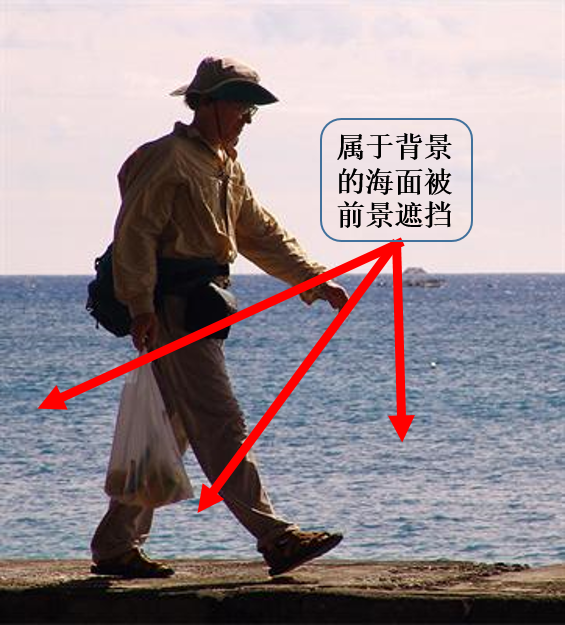
\includegraphics[width=0.4\textwidth]{ch2/occ1.png}}%
 \hspace{1em}%
  \subcaptionbox{其它遮挡情况\label{fig:sub:occ2}}
      {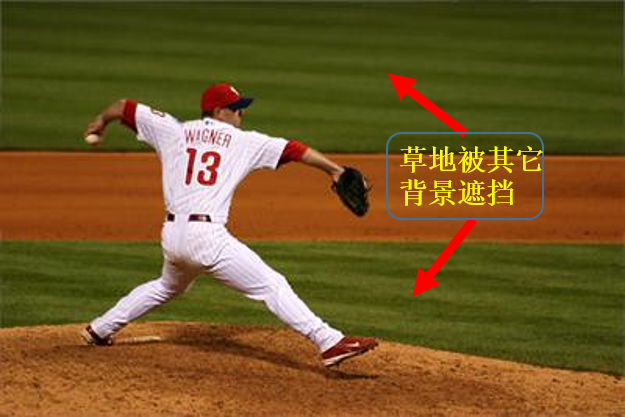
\includegraphics[width=0.4\textwidth]{ch2/occ2.png}}

  \caption{遮挡示例}
  \label{fig:occ}
\end{figure}

\renewcommand{\algorithmcfname}{算法}
\begin{algorithm}[!htbp]
\caption{遮挡处理}
\label{alg:algMergeP2}
%注意label要在caption后面否则引用的时候编号不对
\LinesNumbered
\KwData {图像区域$Regions$, 合并门限$Threshold$ }
\KwResult {合并后的区域$Regions$}
    计算$Regions$中的各区域之间的平均颜色直方图距离$avgDist$\;
    //寻找颜色直方图距离最小的两个区域$minI,minJ$\;
    $minDist = FindMinDist(Regions,minI,minJ)$\;
    $MaxDist = avgDist \times Threshold$\;
    \While{$minDist < MaxDist and Size(Regions)>2$}{
	   合并$minI, minJ$\;
        更新$Regions$\;
        $minDist =FindMinDist(Regions,minI,minJ)$\;}



\end{algorithm}
\par

图像中存在局部小区域,因为与周围邻域色彩分布差别较大,造成优先级低无法参与合并。这些区域将形成空洞,如图~\ref{fig:hole}所示。在图~\ref{fig:sub:hole1}中为输入待处理图像,图像中的显著性前景是小狗,背景部分主要包括草地和小花朵,图~\ref{fig:sub:hole2}中为经过第一阶段合并后得到的区域分割结果,其中用不同颜色标注不同区域。从图~\ref{fig:sub:hole2}中可以看出,因为花朵部分在色彩上与草地区域差距较大,这部分区域没有参与到区域合并中,从而形成了空洞。实际上这些空洞小区域对前景区域和背景区域的合并和分离影响并不大,在处理时将其与其合并优先级最高的邻居区域合并。注意到空洞可能出现在背景以及前景区域,在处理时将其与周围邻域最接近的区域合并可以降低区域复杂度,使得前景区域更容易从背景中分离出来。
\begin{figure}[htb]
  \centering%
  \subcaptionbox{输入图像\label{fig:sub:hole1}} %标题的长度,超过则会换行,如下一个小图。
    {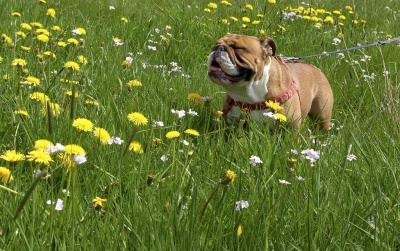
\includegraphics[width=0.4\textwidth]{ch2/hole1.jpg}}%
 \hspace{1em}%
  \subcaptionbox{第一阶段区域合并结果\label{fig:sub:hole2}}
      {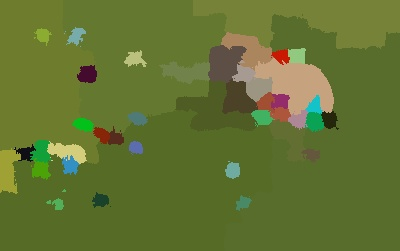
\includegraphics[width=0.4\textwidth]{ch2/hole2.jpg}}

  \caption{空洞示意图}
  \label{fig:hole}
\end{figure}

\subsection{显著性引导的区域合并}
\label{subsec:mergeP3}

在前两个阶段完成后,图像中属于同一对象的像素已经合并到了同一个区域中。第三阶段合并的目标是继续进行区域合并,将图像分为显著性区域和背景区域。与其它大部分基于显著性对象独特性算法不同,本章算法从背景线索入手,不断地将显著性低的区域合并到背景区域。根据观察和实验验证,属于背景的区域主要特点有:
\begin{itemize}
\item (a)连续性强,与周围区域相似度高~\cite{geodesicDistance};
\item (b)靠近图像的边缘~\cite{backgroundPrior};
\item (c)背景区域之间的对比度相对于前景对象较低~\cite{geodesicDistance}。
\end{itemize}

根据(a)和(b),可以推断背景区域易在第一阶段和第二阶段的合并中被合并到包含图像边缘的区域中。因此,选取包含图像边缘像素最多的区域作为背景区域$R_B$。定义区域的显著性值为:
\begin{equation}
   \label{equ:chap2:Saliency}
   Saliency(i)=k_b \times (1-BorderR(i))+ k_a \times (1-AD2C(i)) + k_c \times ContrastB(i)
\end{equation}
其中,$BorderR(i)$表示区域$i$中属于图像边缘的像素占全部图像边缘的比例,$ContrastB(i)=HistogranDist(H(i),H(R_B ))$,即区域$i$与背景区域$R_B$的颜色直方图距离。 $AD2C(i)$为区域$i$中心与图像中心的平均距离,归一化到$[0,1]$范围。在大多数情况下,摄影师在拍摄照片时都会将主体放在靠近中心的位置,因此靠近图像边缘的部分是背景的概率较大。加权系数$k_b,k_a,k_c$为常量,它们的值分别为0.3、0.3、0.4。\par
第三阶段合并的算法如算法~\ref{alg:algMergeP3}所示。
\renewcommand{\algorithmcfname}{算法}
\begin{algorithm}[htb]
\LinesNumbered
\KwData {图像区域$Regions$, 背景区域$R_B$ }
\KwResult {候选显著性区域Proposals}

    \While{$Size(Regions)>2$}{
	   利用公式\ref{equ:chap2:Saliency}计算$Regions$中每个区域$i$的显著性值$S(i)$\;
        寻找显著性值最小的区域$minR$\;
        将$minR$合并到$R_B$\;
        $Proposal = \forall R \in Regions, R \neq  R_B$ \;
        将$Proposal$添加到$Proposals$\;}

\caption{显著性引导的区域合并}
\label{alg:algMergeP3}

\end{algorithm}
\par
在图~\ref{fig:sgrm}中展示了一个显著性引导的区域合并的例子。在图~\ref{fig:sgrm}(a)中是图~\ref{fig:sub:img}经过前两个阶段区域合并后的结果,用不同随机颜色填充不同区域,下同。图~\ref{fig:sgrm}(b)-(h)为显著性引导区域合并的过程。在每次合并时,将当前显著性最弱的区域合并到背景区域,直到只剩2个区域。从图中可以看到,显著性对象直到合并的最后阶段才被合并到背景区域中。虽然合并的最终目标是得到显著性对象和背景两个区域,但是实际上却很难实现。主要原因是在自然图像中,显著性前景自身可能由多个齐次性区域组成,例如图~\ref{fig:sub:img}中的划船人。在实验中,作者发现将显著性对象的各部分合并在一起是十分困难的,主要受到到显著性对象的复杂度和不确定性影响的干扰。因此本章提出以显著性引导的方式,不断将显著性弱的区域合并到背景。合并过程中产生的中间结果以及合并顺序等信息可以用来计算准确的显著性对象区域。

\begin{figure}[htb]
  \centering%
      {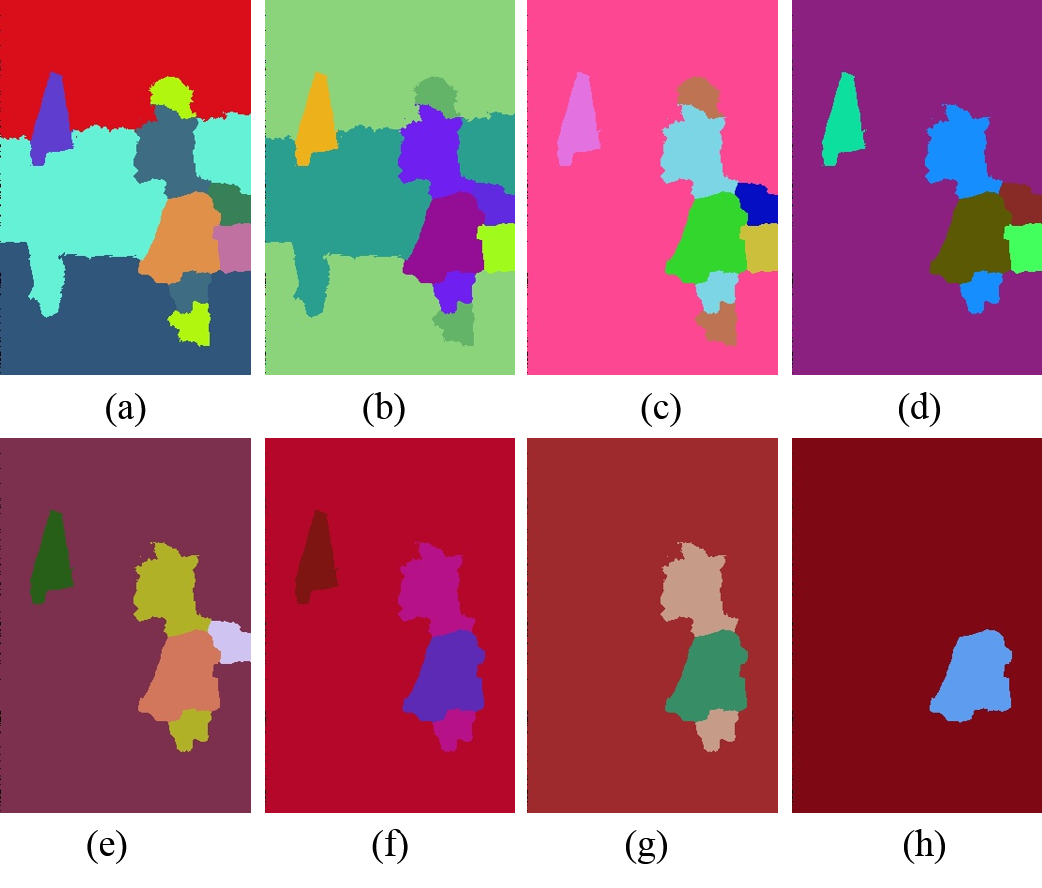
\includegraphics[width=0.9\textwidth]{ch2/sgrm.png}}\\

  \caption{显著性引导的区域合并示意图}
  \label{fig:sgrm}
\end{figure}

\par
\subsection{显著性区域检测}
\label{subsec:saliency}

在自然图像中,前景通常可认为是由多个部分组成,例如人的身体通常可分为皮肤部分、衣服、裤子等。这些部分的颜色和纹理信息等有着较大差别,在合并时很难合并到一起。例如,在图~\ref{fig:sub:fig}中为两幅输入待处理图像,从图像中可以看出上方图像中的显著性对象为红色花朵,下方图像中的显著性对象为两个散步的人。图~\ref{fig:sub:seg}中为经过前两个阶段区域合并后的结果。从图~\ref{fig:sub:fig}中我们看到,经过区域分割之后更容易提取显著性对象。特别是上方图像中的花朵,在区域合并时被分在一个区域,通过比较区域的显著性很容易将其从背景中提取出来。但是,下方图像中的情况更为复杂,从图中易知前景对象是两个穿不同颜色衣裤的人,但是在区域合并时无法将所有属于前景的区域合并在一起。这时,所求显著性对象分布在5个区域之中。

\begin{figure}[htb]
  \centering%
  \subcaptionbox{输入图像\label{fig:sub:fig}} %标题的长度,超过则会换行,如下一个小图。
    {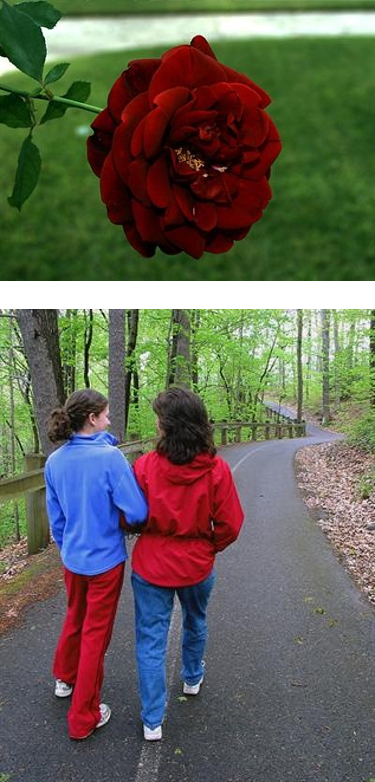
\includegraphics[width=0.25\textwidth]{ch2/fig.png}}%
 \hspace{1em}%
  \subcaptionbox{区域合并结果\label{fig:sub:seg}}
      {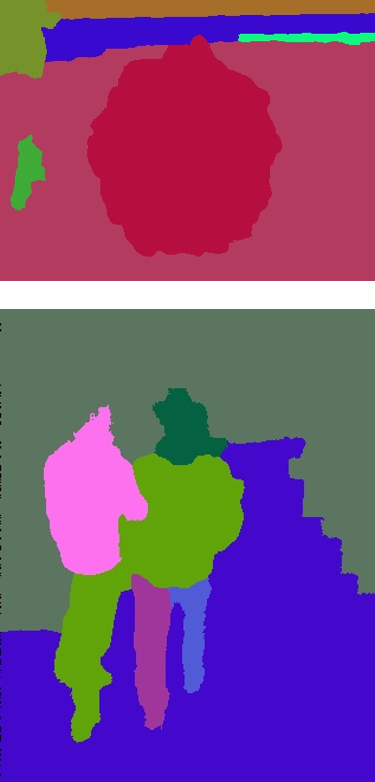
\includegraphics[width=0.25\textwidth]{ch2/seg.png}}

  \caption{齐次的前景区域可以合并到一个区域并易于提取,而非齐次前景对象在区域合并后可能包含多个区域。}
  \label{fig:fgseg}
\end{figure}

\par
为了得到完整的显著性区域,本章算法将第三阶段合并过程中产生的非背景区域作为候选显著性区域(proposals)。假设候选区域$Proposals(i)$包括$k_i$个区域,其中区域$j$的显著性值$PropSal(i,j)$定义为:
$$
   PropSal(i,j)=ContrastB(j) \times \exp{(-\frac{Ad2c(j)^2}{\varphi_d^2 })}
$$
其中,$\varphi_d=0.33$为固定值。\par
在合并过程中可以得到多个候选显著性区域,综合考虑候选区域的对比度、形状以及大小等因素对每个候选区域进行可靠性评估,其可靠性值定义为:
\begin{equation}
   \label{equ:chap2:PropSal}
   PropCon(i,j)=w_o \times Obj(i) + w_f \times Fillness(i) + w_{sc} \times Scale(i)
\end{equation}
其中, $Obj(i)$用于评估区域中包含对象的可能性(Objectness)\cite{objectness},具体定义为:
$$Obj(i) = HistogramDist(H(i),H(BoxBorder(i)))$$
设$BB(i)$为包围$Proposals(i)$的最小矩形.上式中$H(BoxBorder(i))=Histogram(p), p \in BB(i)-Proposals(i)$,表示位于$BB(i)$之内区域$Proposals(i)$之外的边界部分像素的直方图。公式\ref{equ:chap2:PropSal}中的$Fillness$定义为:
$$ Fillness(i) = \exp({-(\frac{size(i)}{size(BB(i))}-m_f)^2}/\varphi_f^2)$$ \par

在一般情况下,显著性区域一般形状较为紧凑,假如候选区域中还包括背景区域则会使得$Fillness$值较小。本章中$m_f,\varphi_f$分别为0.56和0.33。 公式\ref{equ:chap2:PropSal}中的最后一项为尺度可靠性,定义为$Scale(i)= \exp(-(size(i)- m_s)^2/\varphi_s^2)$,主要评估显著性区域大小的可靠性,在大多数情况下显著性区域一般只占整个图像的局部,假如候选区域过大则说明其中还包括未合并到背景中的非显著性区域;而如果候选区域过小则说明其可能仅是前景的一部分。本章中$m_s,\varphi_s$分别为0.3和0.5。\par

最后,依据$P$个候选显著性区域及其可靠性指标,以加权平均的方式得到最终显著性结果:
$$ S(I) = \frac{\sum_{i=1}^{P}PropCon(i) \times \sum_{j=1}^{k_i}PropSal(i,j)}{\sum_{i=1}^{P}PropCon(i)}$$

上述过程如图~\ref{fig:weighted}所示,其中将候选显著性区域的可靠性值量化到[0,255]之间,以灰度图格式显示。经过图~\ref{fig:weighted}中左侧的候选显著性区域加权后得到的最终结果如右侧所示。以加权平均的方式计算最终的显著性区域结果可以处理显著性对象分布在多个区域的情况,相比于提取单个显著性区域或者尝试将显著性区域合并到一个区域的方法,该算法的鲁棒性更好。
\begin{figure}[htb]
  \centering%
      {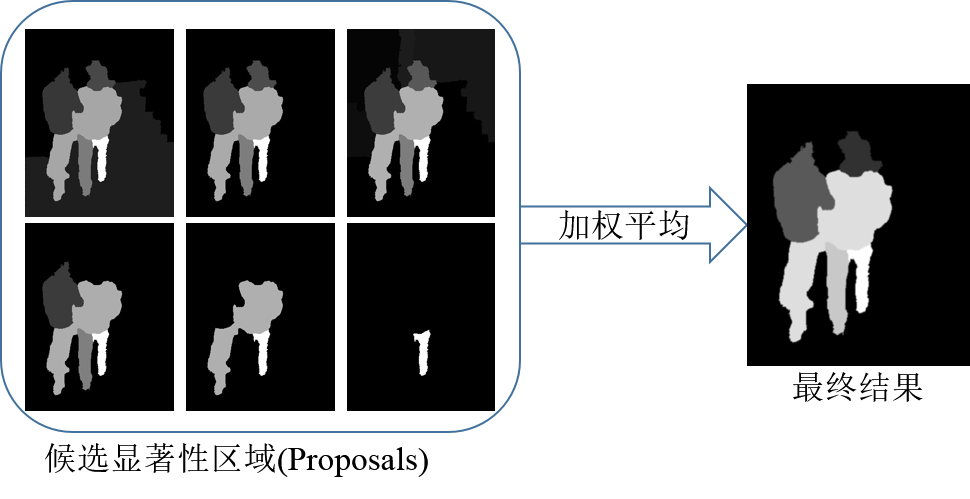
\includegraphics[width=0.9\textwidth]{ch2/weighted.png}}\\

  \caption{显著性引导的区域合并示意图}
  \label{fig:weighted}
\end{figure}

\section{实验结果与分析}
\label{sec:results}


通过C++编程借助OpenCV~\cite{opencv_library}实现了本文算法,在两个公开的测试集ASD~\cite{Achanta08}和ECSSD~\cite{ECSSD}上进行了测试。两个数据集中均包含1000张图像。其中ECSSD数据集中的图像主要是自然场景下拍摄的图像,其背景复杂度相比于ASD数据集中的图像更高,同时也更接近日常实际应用。这两个数据集中均包含人工标注的精确显著性区域。\par
在实验中, 算法~\ref{alg:algMergeP1}中的参数设置为$k=0.2,N=15$,算法~\ref{alg:algMergeP2}中的$threshold=0.8$。公式~\ref{equ:chap2:PropSal}中的系数$w_o,w_f,w_{sc}$分别为0.3、0.05、0.65,在本章所以实验中上述所有参数均使用固定值。

\subsection{显著性检测}
\label{sec:sub:saliencyRst}

为验证本章算法在显著性区域检测中的有效性,将本章所提出的算法 (RM)与AC~\cite{Achanta08}、CHS~\cite{Yan2014Hierarchical}、FT~\cite{saliencyFilter}、GB~\cite{Harel07graph-basedvisual}、GC~\cite{GC},GMR~\cite{GMR},IT~\cite{itti},RC~\cite{ChengPAMI}, SF~\cite{saliencyFilter}、SR~\cite{SR}、DSR~\cite{DSR}、PISA~\cite{PISA}、MC~\cite{MC}等方法进行了比较。其中RC、GMR、CHS、MC算法和本文算法都属于基于区域的方法。部分结果的比较见图~\ref{fig:chap2:comp1}和图~\ref{fig:chap2:comp2},由于早期的AC、IT、SR等算法准确度较低,在图~\ref{fig:chap2:comp1}和图~\ref{fig:chap2:comp2}中只列出了效果更好的6种算法的结果通过对比可以看到,本章算法可以处理各种复杂背景的自然图像,例如图~\ref{fig:chap2:comp1}中的第三行以及图~\ref{fig:chap2:comp2}中的第二行,对于这些类型的图像RC等算法无法有效工作。而对于背景部分与前景部分在色彩空间分布较为接近的情况,例如图~\ref{fig:chap2:comp1}中的第二行及图~\ref{fig:chap2:comp2}中的第三行,本文算法的处理结果同样优于基于全局对比度的RC等算法。\par
\begin{figure}[h]
  \centering%
      {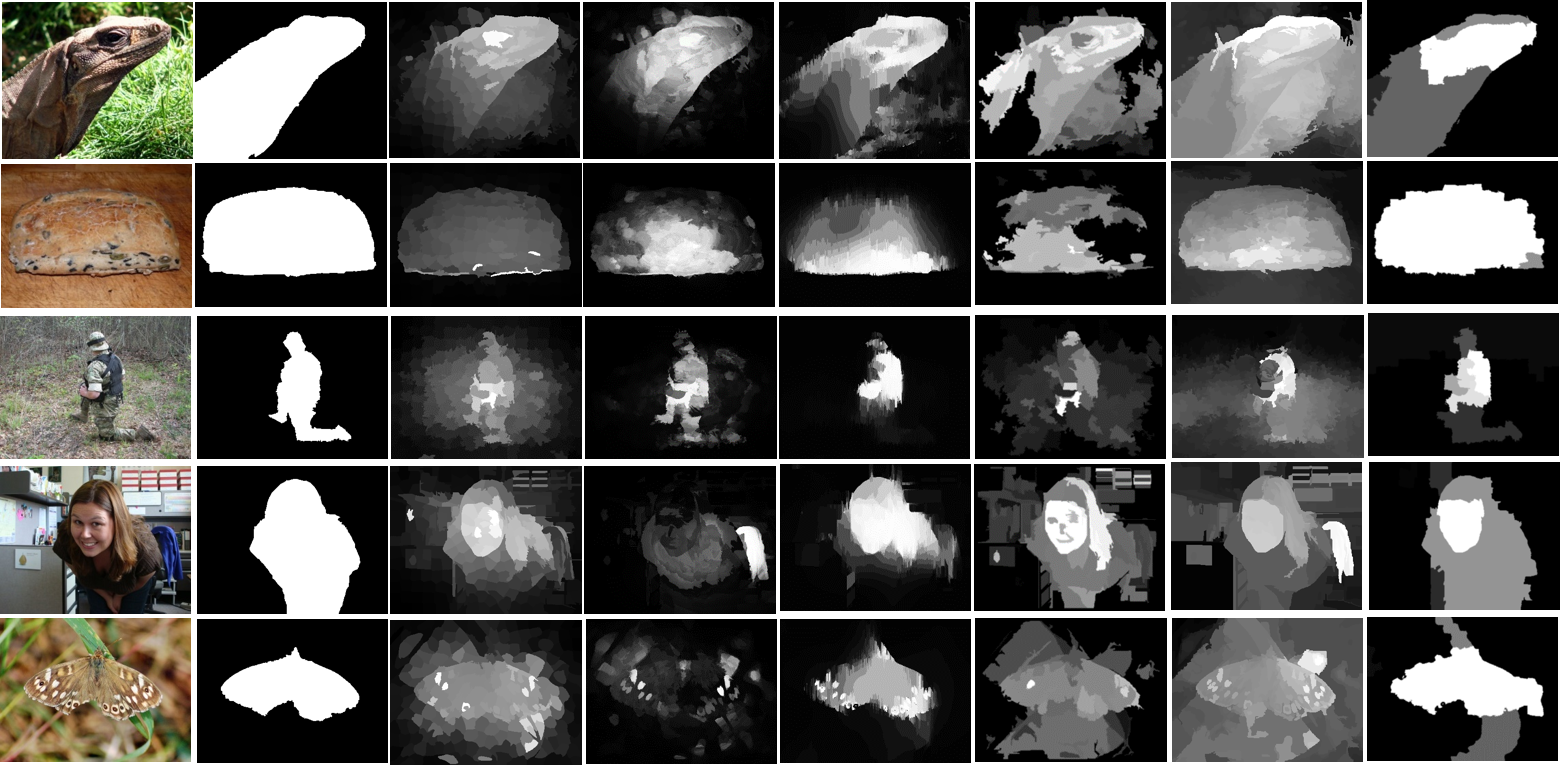
\includegraphics[width=1\textwidth]{ch2/ECSSDRes.png}}\\
(a)输入 (b)正确结果(c)MC \quad (d) DSR \quad (e) PISA \quad (f)RC \quad (g)CHS \quad (h)RM\\
  \caption{ECSSD数据集部分图像显著性检测结果比较}
  \label{fig:chap2:comp1}
\end{figure}
\begin{figure}[h]
  \centering%
      {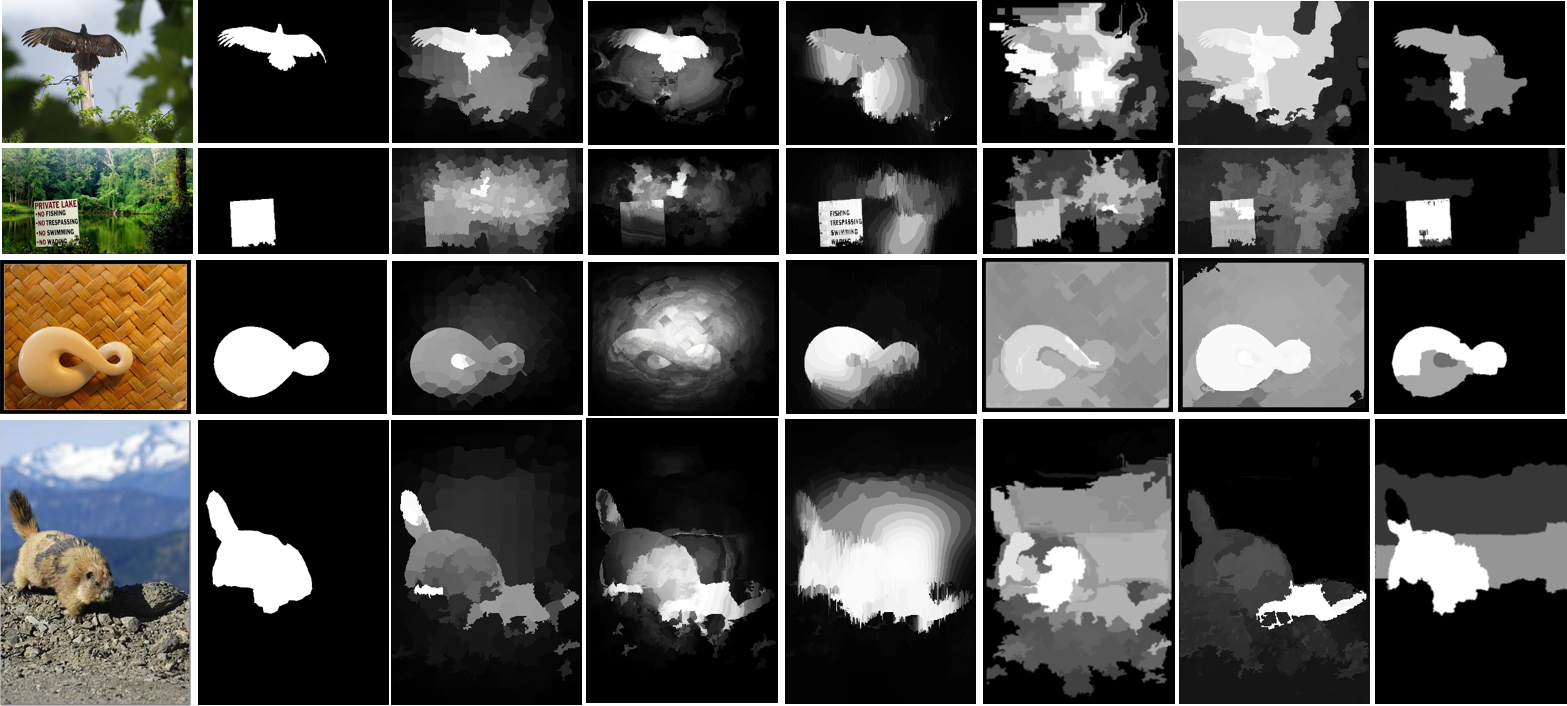
\includegraphics[width=1\textwidth]{ch2/ASDRes.png}}\\
(a)输入 (b)正确结果(c)MC \quad (d) DSR \quad (e) PISA \quad (f)RC \quad (g)CHS \quad (h)RM\\
  \caption{ASD数据集部分图像显著性检测结果比较}
  \label{fig:chap2:comp2}
\end{figure}
为了定量衡量算法的准确性,将显著性检测结果进行二值化后得到的显著性对象与数据集中提供的正确结果进行对比,本文采用通用的F-Measure值指标来比较算法准确性,其定义为:
$$F_{\beta} = \frac{(1+\beta^2)Precision \times Recall}{\beta^2 \times Precision + Recall}$$
其中$Precision$为精度,$Recall$表示召回率,$\beta^2=0.3$. \par

在实验中,为了消除二值化阈值对结果的影响,将阈值设定为在0到255之间变化,绘制F-Measure随阈值变化的曲线,见图~\ref{fig:sub:ecssdFCurve}和图~\ref{fig:sub:asdFCurve},同时图~\ref{fig:sub:ecssdAvg},~\ref{fig:sub:asdAvg}统计了各方法得到的F-Measure平均值和最大值。通过比较可以看出,本章算法在ECSSD数据集中的F-Measure平均值和最大值略微大于PISA算法,且均优于其他算法, 在ASD数据集中得到的最大F-Measure为0.89, 略低于最高的MC算法(0.91)。 本文算法得到的F-Measure曲线较为扁平, 即F-Measure取值受阈值影响较小, 当阈值门限在128附近时F-Measure可以得到最大值。 比较两个数据集,可以发现ASD数据集中的部分图像背景复杂度较低,因此各算法在ASD数据集上的测试结果均优于ECSSD数据集上的结果。由于本章算法的结果是通过基于超像素的区域合并得到的,显著性值的最小计算单元为超像素,这使得本文算法在ASD数据集中得到的结果的精度要略低于GMR、PISA等算法。 \par
$MAE$是另一个衡量显著性区域检测结果准确性的指标,其定义为:
$$MAE=1/(W\times H) \sum_{x=1}^W\sum_{y=1}^H \| S(x,y)-G(x,y)\|$$ ,其中$W,H$分别为图像的宽和高,$S$为显著性检测结果,$G$为正确值,两者均归一化在[0,1]之间。MAE值越低说明显著性检测误差越小,图~\ref{fig:MAERst}是各算法MAE值在两个数据库中的比较结果。本文算法同样在ECSSD数据库中优于其它算法,在ASD数据库中略高于MAE最低的PISA算法。\par
\begin{figure}[h]
  \centering%
  \subcaptionbox{F-Measure曲线\label{fig:sub:ecssdFCurve}} %标题的长度,超过则会换行,如下一个小图。
    {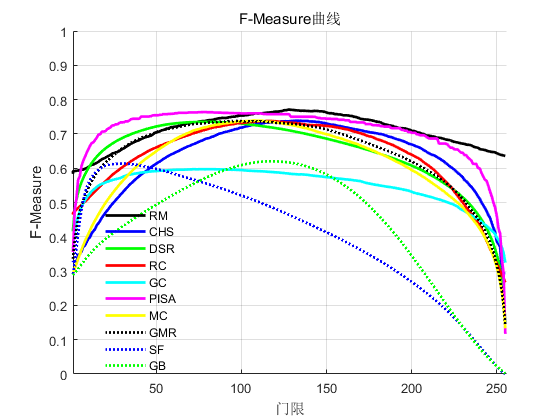
\includegraphics[width=0.45\textwidth]{ch2/FCurve_ECSSD}}%
 %\hspace{1em}%
  \subcaptionbox{平均F-Measure\label{fig:sub:ecssdAvg}}
      {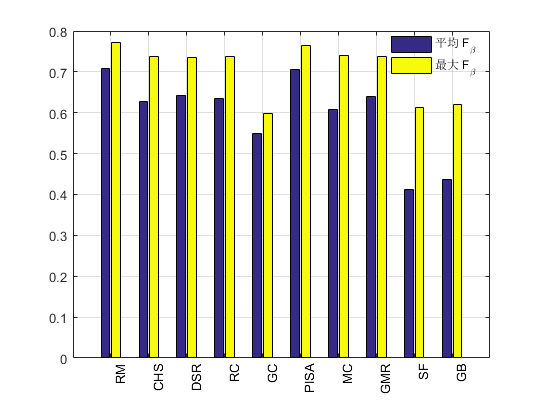
\includegraphics[width=0.45\textwidth]{ch2/FMeasure_ECSSD.png}}
  \caption{ECSSD数据库F-Measure值比较}
  \label{fig:ECSSDRst}
\end{figure}

\begin{figure}[h]
  \centering%
  \subcaptionbox{F-Measure曲线\label{fig:sub:asdFCurve}} %标题的长度,超过则会换行,如下一个小图。
    {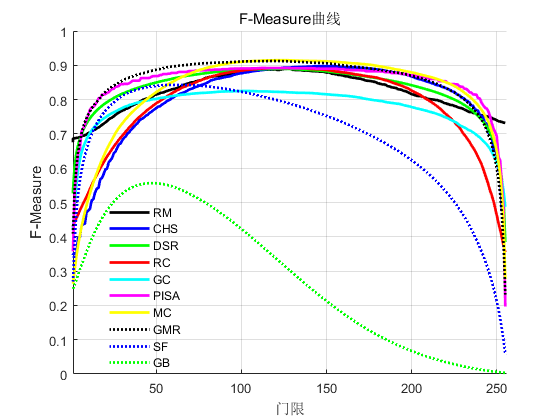
\includegraphics[width=0.45\textwidth]{ch2/FCurve_ASD}}%
 %\hspace{1em}%
  \subcaptionbox{平均F-Measure\label{fig:sub:asdAvg}}
      {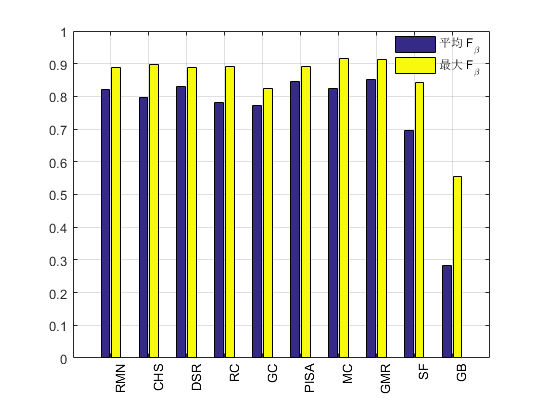
\includegraphics[width=0.45\textwidth]{ch2/FMeasure_ASD.png}}
  \caption{ASD数据库F-Measure值比较}
  \label{fig:ASDRst}
\end{figure}

\begin{figure}[h]
  \centering%
  \subcaptionbox{ECSSD数据集结果\label{fig:sub:ecssdMAE}} %标题的长度,超过则会换行,如下一个小图。
    {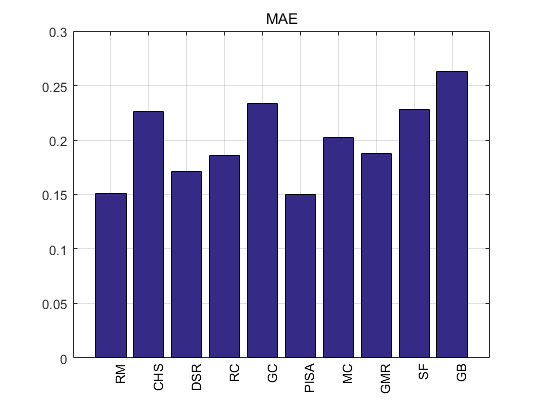
\includegraphics[width=0.45\textwidth]{ch2/ECSSD_MAE.png}}%
 %\hspace{1em}%
  \subcaptionbox{ASD数据集结果\label{fig:sub:asdMAE}}
      {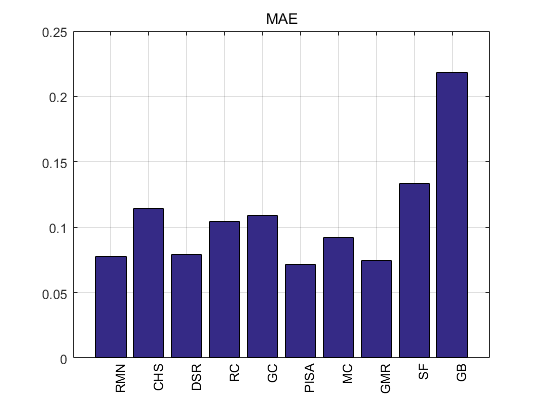
\includegraphics[width=0.45\textwidth]{ch2/ASD_MAE.png}}
  \caption{算法MAE比较}
  \label{fig:MAERst}
\end{figure}

部分算法的速度比较见表~\ref{tab:algTime}.所列数据在配备Intel i7 3.5GHz CPU,16GB RAM的电脑上测得,参与比较的算法均用C++语言实现,其中CHS,RC和GMR算法均使用作者公开的代码进行测试。ASD数据库和ECSSD数据库中图像大小平均约为$400 \times 300$,表中所列时间为处理每幅图像所用的平均时间。本章算法的速度相比RC和GMR算法稍快,比CHS算法快4倍左右,比与本章算法准确度接近的PISA快7倍左右。\par

\begin{table}[htb]
  \centering

  \caption{算法时间比较}
  \label{tab:algTime}
    \begin{tabularx}{\linewidth}{lXXXXX}
      \toprule[1.5pt]
      {\heiti 算法} & {\heiti RM} & {\heiti CHS} & {\heiti RC} & {\heiti GMR} &{\heiti PISA}\\\midrule[1pt]
      时间(s) & {\bf 0.084} & 0.362 & 0.091 & 0.097&0.583 \\

      \bottomrule[1.5pt]
    \end{tabularx}

\end{table}

\subsection{图像分割结果}
\label{sec:sub:segmentation}

本章所提算法通过区域合并的方式逐渐将图像中相似区域进行合并,在合并过程中可以得到一系列图像分割结果。这些图像分割结果可以为显著性前景检测,对象定位等应用提供重要线索。在本节中,将本章算法与其它图像区域分割算法~\cite{Richard2004Statistical,Xiao2015Complexity,MeanShift}进行比较。在实验中,将图像分割目标设为10。利用各算法进行图像分割时有时不能保证正好得到10个区域,这时选取最接近目标的分割结果作为最终结果。一个好的图像分割算法可以将感兴趣区域其中在一个区域,并且与背景区域分开。如果分割结果所包含的区域过多则包含较多冗余信息,过少则会使得前景区域合并到背景区域中,无法准确提取显著性对象。因此实验中将分割目标设为10左右,基本能同时满足简化图像结构以及保持显著性对象边界的目标。\par
实验中部分比较结果如图~\ref{fig:segCom}所示,其中(a)列图像为输入图像,(b)-(e)列分别为SRM、文献~\inlinecite{Xiao2015Complexity}、Mean Shift~\cite{MeanShift},以及本章算法的分割结果。通过比较可以看出,本章算法的分割结果基本上能够避免将前景对象合并到背景中。而其它图像分割算法均存在将前景对象合并到背景中的情况。主要原因在于这些图像区域分割算法~\cite{Richard2004Statistical,Xiao2015Complexity,MeanShift}在分割时没有考虑到分割过程中不同阶段的特点,始终以同样的策略进行区域合并。另外,在合并过程中没有对遮挡和空洞等情况进行特殊处理。\par
综上所述,本章提出的显著性引导的区域合并算法能够在图像分割过程中较好的保持前景对象的边界,避免其合并到背景区域;同时经过遮挡和空洞处理后,背景区域也可以合并到一起降低了复杂度,有助于显著性前景的提取。
\begin{figure}[htb]
  \centering%
      {\includegraphics[width=0.9\textwidth]{ch2/segcom.png}}\\

  \caption{图像分割效果比较,(a)输入图像,(b)SRM~\cite{Richard2004Statistical},(c)文献~\inlinecite{Xiao2015Complexity},(d)Mean Shift~\cite{MeanShift},(e)本章算法}
  \label{fig:segCom}
\end{figure}


\subsection{算法失败的情况}
\label{subsec:failure}

虽然本章算法可以处理部分复杂背景的情况,但在处理背景连续性较差的图像时效果较差。主要原因是在区域合并的过程中会将前景区域错误的合并到背景中,从而无法提取到正确的前景。例如,在图~\ref{fig:fail}中,前两列为输入图像和正确前景,后三列分别为本文算法第一阶段,第二阶段合并结果以及最终提取的显著区域结果。由于这两幅图像中的背景部分十分复杂,并不具备本文假设的连续性。因此在区域合并时误将前景区域合并到了背景中,从而导致算法无法提取正确的显著性前景。
 \begin{figure}[htb]
  \centering%
      {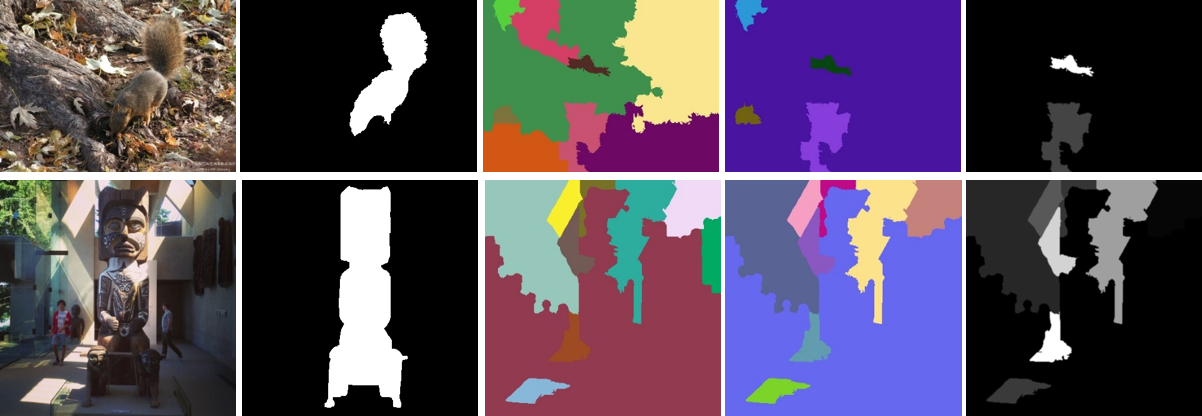
\includegraphics[width=0.9\textwidth]{ch2/fail.png}}

  \caption{本章算法部分失败例子}
  \label{fig:fail}
\end{figure}


\section{本章小结}
图像显著性区域检测是当前计算机视觉相关领域备受关注的研究热点区域之一。准确提取图像中显著性对象对于图像的识别和理解来说是重要的第一步。虽然人类视觉系统与生俱来就具备这种能力,但是在计算机上实现达到甚至超越人类视觉系统的识别准确度的显著性检测算法却较为困难。虽然近些年提出的一些算法大大提高了图像显著性检测算法的效率和准确度~\cite{ChengPAMI,ufo,Yan2014Hierarchical,geodesicDistance},但是对于一些困难的情况,例如背景复杂度高、前景与背景相近等,目前已有的算法仍无法得到令人满意的结果。\par
本章对图像显著性检测问题进行了研究。借助图像背景线索,以将图像分为显著性对象和背景2个区域为目标,提出了一种基于区域合并的显著性检测算法。由于在区域合并的不同阶段采取了不同的合并策略,本章算法能有效的防止在合并过程中将前景显著性对象错误的合并到背景区域。同时,为了得到准确的显著性对象,本章算法利用背景线索进行区域显著性分析,不断将非显著性区域合并到背景区域。最后,将合并过程中得到的非背景区域作为候选显著性区域,通过加权平均的方式得到最终结果。区别于当前主流算法的主要思路,本章算法采用了基于背景的线索和图像合并的方式提取显著性对象。与前景线索相比,背景线索的通用性更强。图像中的前景对象特征会随着图像内容和应用场景的变化而千变万化,而图像背景部分所具备的连续性强等特点却不会随着图像内容而变化。\par
为了验证本章算法那的有效性,在2个公开数据集上测试了本章所提出的算法。实验结果证明了本章所提算法的有效性。在主要是由自然图像构成,难度较大的ECSSD数据集上的实验中,本章算法的准确度和误差指标均优于其他参与比较的算法。本章算法简单直观,且效率高,且易于实现。\par
由于本章所提算法主要基于背景的连续性特点。针对背景连续性不足的图像,目前本章算法无法有效的通过区域合并将背景部分合并在一起,同时可能会将前景错误的合并到背景中。为解决这一问题,在下一步的工作中将考虑引入色彩相似性之外的其它度量方式以及多尺度分析方法来更好的评估图像背景区域之间的相似性。
